\documentclass[11pt]{scrartcl} % Font size
%%%%%%%%%%%%%%%%%%%%%%%%%%%%%%%%%%%%%%%%%
% Wenneker Assignment
% Structure Specification File
% Version 2.0 (12/1/2019)
%
% This template originates from:
% http://www.LaTeXTemplates.com
%
% Authors:
% Vel (vel@LaTeXTemplates.com)
% Frits Wenneker
%
% License:
% CC BY-NC-SA 3.0 (http://creativecommons.org/licenses/by-nc-sa/3.0/)
% 
%%%%%%%%%%%%%%%%%%%%%%%%%%%%%%%%%%%%%%%%%

%----------------------------------------------------------------------------------------
%	PACKAGES AND OTHER DOCUMENT CONFIGURATIONS
%----------------------------------------------------------------------------------------

\usepackage{amsmath, amsfonts, amsthm} % Math packages
\usepackage[stable]{footmisc}
\usepackage{listings} % Code listings, with syntax highlighting

 % English language hyphenation

\usepackage{graphicx} % Required for inserting images
\graphicspath{{Figures/}{./}} % Specifies where to look for included images (trailing slash required)

\usepackage{booktabs} % Required for better horizontal rules in tables

\numberwithin{equation}{section} % Number equations within sections (i.e. 1.1, 1.2, 2.1, 2.2 instead of 1, 2, 3, 4)
\numberwithin{figure}{section} % Number figures within sections (i.e. 1.1, 1.2, 2.1, 2.2 instead of 1, 2, 3, 4)
\numberwithin{table}{section} % Number tables within sections (i.e. 1.1, 1.2, 2.1, 2.2 instead of 1, 2, 3, 4)

\setlength\parindent{0pt} % Removes all indentation from paragraphs

\usepackage{enumitem} % Required for list customisation
\setlist{noitemsep} % No spacing between list items

\usepackage{color}

%----------------------------------------------------------------------------------------
%	DOCUMENT MARGINS
%----------------------------------------------------------------------------------------
\usepackage[utf8]{vietnam}
\usepackage[english]{babel}
\usepackage[utf8]{inputenc}
\usepackage{geometry} % Required for adjusting page dimensions and margins

\geometry{
	paper=a4paper, % Paper size, change to letterpaper for US letter size
	top=2.5cm, % Top margin
	bottom=3cm, % Bottom margin
	left=3cm, % Left margin
	right=3cm, % Right margin
	headheight=0.75cm, % Header height
	footskip=1.5cm, % Space from the bottom margin to the baseline of the footer
	headsep=0.75cm, % Space from the top margin to the baseline of the header
	%showframe, % Uncomment to show how the type block is set on the page
}

%----------------------------------------------------------------------------------------
%	FONTS
%----------------------------------------------------------------------------------------





%----------------------------------------------------------------------------------------
%	HEADERS AND FOOTERS
%----------------------------------------------------------------------------------------

\usepackage{scrlayer-scrpage} % Required for customising headers and footers

\ohead*{} % Right header
\ihead*{} % Left header
\chead*{} % Centre header

\ofoot*{} % Right footer
\ifoot*{} % Left footer
\cfoot*{\pagemark} % Centre footer
\usepackage[unicode]{hyperref}
 % Include the file specifying the document structure and custom commands
%----------------------------------------------------------------------------------------
%	TITLE SECTION
%----------------------------------------------------------------------------------------
\title{	
	\normalfont\normalsize
	\textsc{VNUHCM - University of Science \\Faculty of Information Technology}\\ % Your university, school and/or department name(s)
	\vspace{25pt} % Whitespace
	\rule{\linewidth}{0.5pt}\\ % Thin top horizontal rule
	\vspace{20pt} % Whitespace
	{\huge Lab01 - Search Problem}\\ % The assignment title
	\vspace{12pt} % Whitespace
	\rule{\linewidth}{2pt}\\ % Thick bottom horizontal rule
	\vspace{12pt} % Whitespace
}

\author{\LARGE 19120212- Vũ Công Duy \\ \LARGE 19120399 - Tô Gia Thuận}
\date{\normalsize\today} % Today's date (\today) or a custom date
\begin{document}
\maketitle 
\begin{figure}[h] % [h] forces the figure to be output where it is defined in the code (it suppresses floating)
	\centering
	
\includegraphics[width=0.4\columnwidth]{hcmus.png} % Example image
\end{figure}

%------------------------------------------------
\section{Xây dựng cấu trúc chương trình} \cite{standfordcs221}
Mục tiêu của việc xây dựng cấu trúc chương trình là để việc cài đặt những thuật toán được tổng quát hóa, giúp cài đặt những bài toán khác nhau và giải chúng bằng nhiều thuật toán khác nhau trở nên đơn giản hơn. 

Theo cách những nhà phát triển phần mềm, mã nguồn có thể được tái sử dụng trong nhiều trường hợp khác nhau, giúp người lập trình có thể tập trung hơn vào phần tối ưu thuật toán mà không nghĩ ngợi nhiều về phần kỹ thuật, cài đặt.

Việc cài đặt dựa chủ yếu vào kỹ thuật kế thừa, đa hình trong kỹ thuật lập trình hướng đối tượng. Chương trình sẽ được trực quan hóa bằng biểu đồ UML sau đây.
\begin{figure}[h] % [h] forces the figure to be output where it is defined in the code (it suppresses floating)
	\centering
	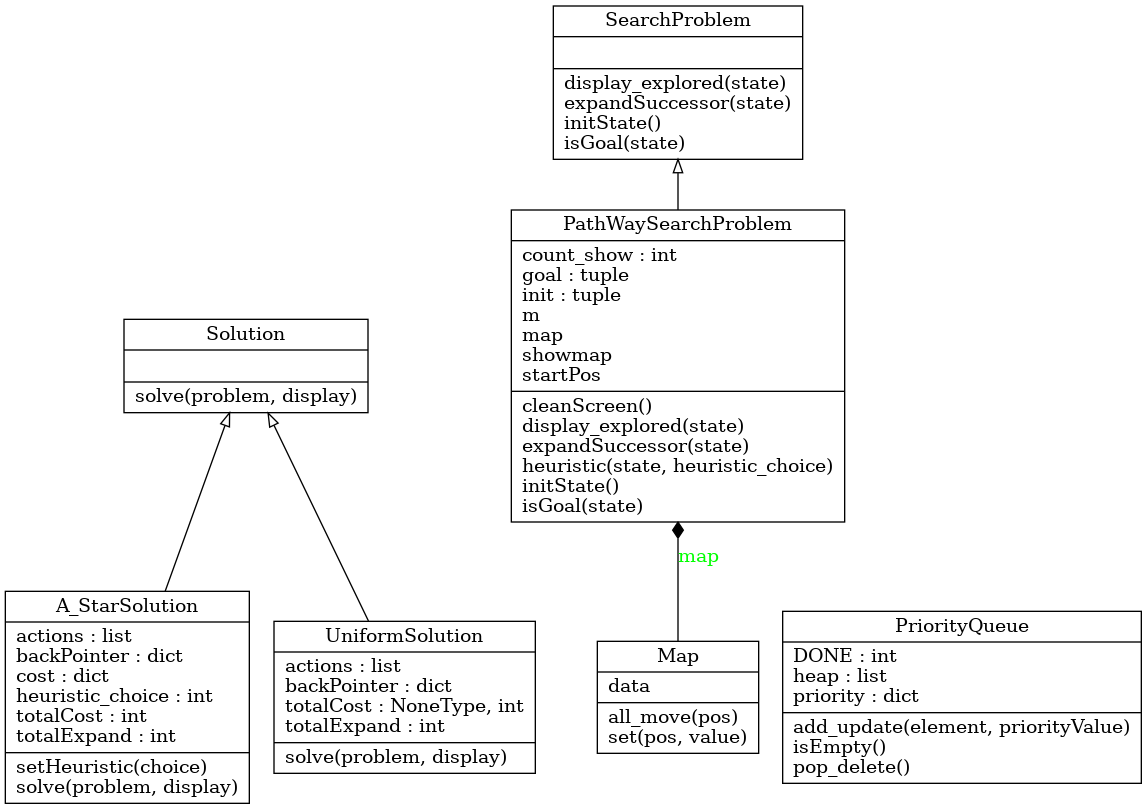
\includegraphics[width=1.2\columnwidth]{classes_uml_diagram.png} % Example image
\end{figure}

\subsection{Hai class trừu tượng (Abstract Class)}
Ở level cao nhất chính là 2 class : Solutimethodon và SearchProblem tương ứng với hai thực thể (entity) là lời giải và bài toán.

Ở abstract class, phương thức (method) sẽ được cài đặt dưới dạng phương thức ảo (virtual method), những phương thức này sẽ được các lớp con kế thừa và được cài đặt trong quá trình viết các lớp con ấy.

Để tránh trường hợp method của abstract class được gọi (có thể do method của class kế thừa chưa được cài đặt), ta sẽ thêm dòng báo lỗi khi method của abstract class được gọi raise NotImplementedError(...)

%------------------------------------------------
\lstinputlisting[
	caption=Cài đặt abstract class, % Caption above the listing
	label=lst:luftballons, % Label for referencing this listing
	language=Perl, % Use Perl functions/syntax highlighting
	frame=single, % Frame around the code listing
	showstringspaces=false, % Don't put marks in string spaces
	numbers=left, % Line numbers on left
	numberstyle=\tiny, % Line numbers styling
	]{abstract_class.txt}

Cấu trúc của bài toán cũng như những "nguyên liệu" để giải bài toán ấy như : trạng thái ban đầu(init state), trạng thái đích(goals), mở rộng trạng thái kề(expand successor)\cite{csttnt_lhb},... được biểu diễn dưới dạng các phương thức của một thực thể của class SearchProblem. Ở class Solution, phương thức duy nhất là solve(problem,display) sẽ được truyền vào tham số là một thực thể của class SearchProblem. Phương thức solve sẽ được cài đặt một cách trừu tượng để có thể giải được bất cứ bài toán tìm kiếm nào dựa vào những "nguyên liệu" được lấy từ thực thể class SearchProblem truyền vào.

Phương thức display\_explored(state) của class SearchProblem có nhiệm vụ trực quan hóa trạng thái hiện tại để quá trình cài đặt thuật toán thuận lợi hơn, không bắt buộc có.Vì vậy, class kế thừa SeachProblem không bắt buộc cài đặt phương thức này, ta cho lệnh "pass" (bỏ qua) nếu phương thức này được gọi từ abstract class.

\subsection{Class PriorityQueue}
Đây là lớp hàng đợi ưu tiên được bổ sung một vài tính năng để tối ưu cho bài toán tìm kiếm.

Các tính năng bổ sung bao gồm : không push lại những phần tử đã được pop, update chỉ số ưu tiên nếu chỉ số ưu tiên mới lớn hơn chỉ số cũ. 
\lstinputlisting[
	caption=Cài đặt class PriorityQueue, % Caption above the listing
	label=lst:luftballons, % Label for referencing this listing
	language=Perl, % Use Perl functions/syntax highlighting
	frame=single, % Frame around the code listing
	showstringspaces=false, % Don't put marks in string spaces
	numbers=left, % Line numbers on left
	numberstyle=\tiny, % Line numbers styling
]{priority_queue.txt}

Thuộc tính \textbf{heap} là một list các tuple (element, value).Việc sắp xếp, pop, push các phần tử theo cấu trúc heap được thực hiện bởi hàm heappush trong thư viện heapq của python3.

Thuộc tính \textbf{priority} là một dict lưu trữ các element đã được thêm vào heap (kể cả các element đã được pop khỏi heap) và value của mỗi element đó. Những element nào đã được pop ra sẽ được gán value bằng với thuộc tính \textbf{DONE} mang giá trị $- \infty$ để phân biệt với các giá trị khác, thuận tiện cho việc viết điều kiện rẽ nhánh cho chương trình bỏ qua update hoặc thêm vào heap nếu đã được pop.
\subsection{Các class kế thừa abstract class}




\bibliographystyle{plain}
\bibliography{ref}
\end{d ocument}
